\section{Estado Actual}
Encontrar información sobre un instrumento suele ser tan sencillo como realizar una búsqueda en internet. En el caso de \textbf{la guitarra y el ukelele}, los recursos son casi ilimitados gracias a la existencia de un gran número de páginas~(véase Figura~\ref{fig:cifra_isadecandidito}) y aplicaciones que cuentan con comunidades que crean y difunden contenido constantemente.

\begin{figure}[H]
    \centering
    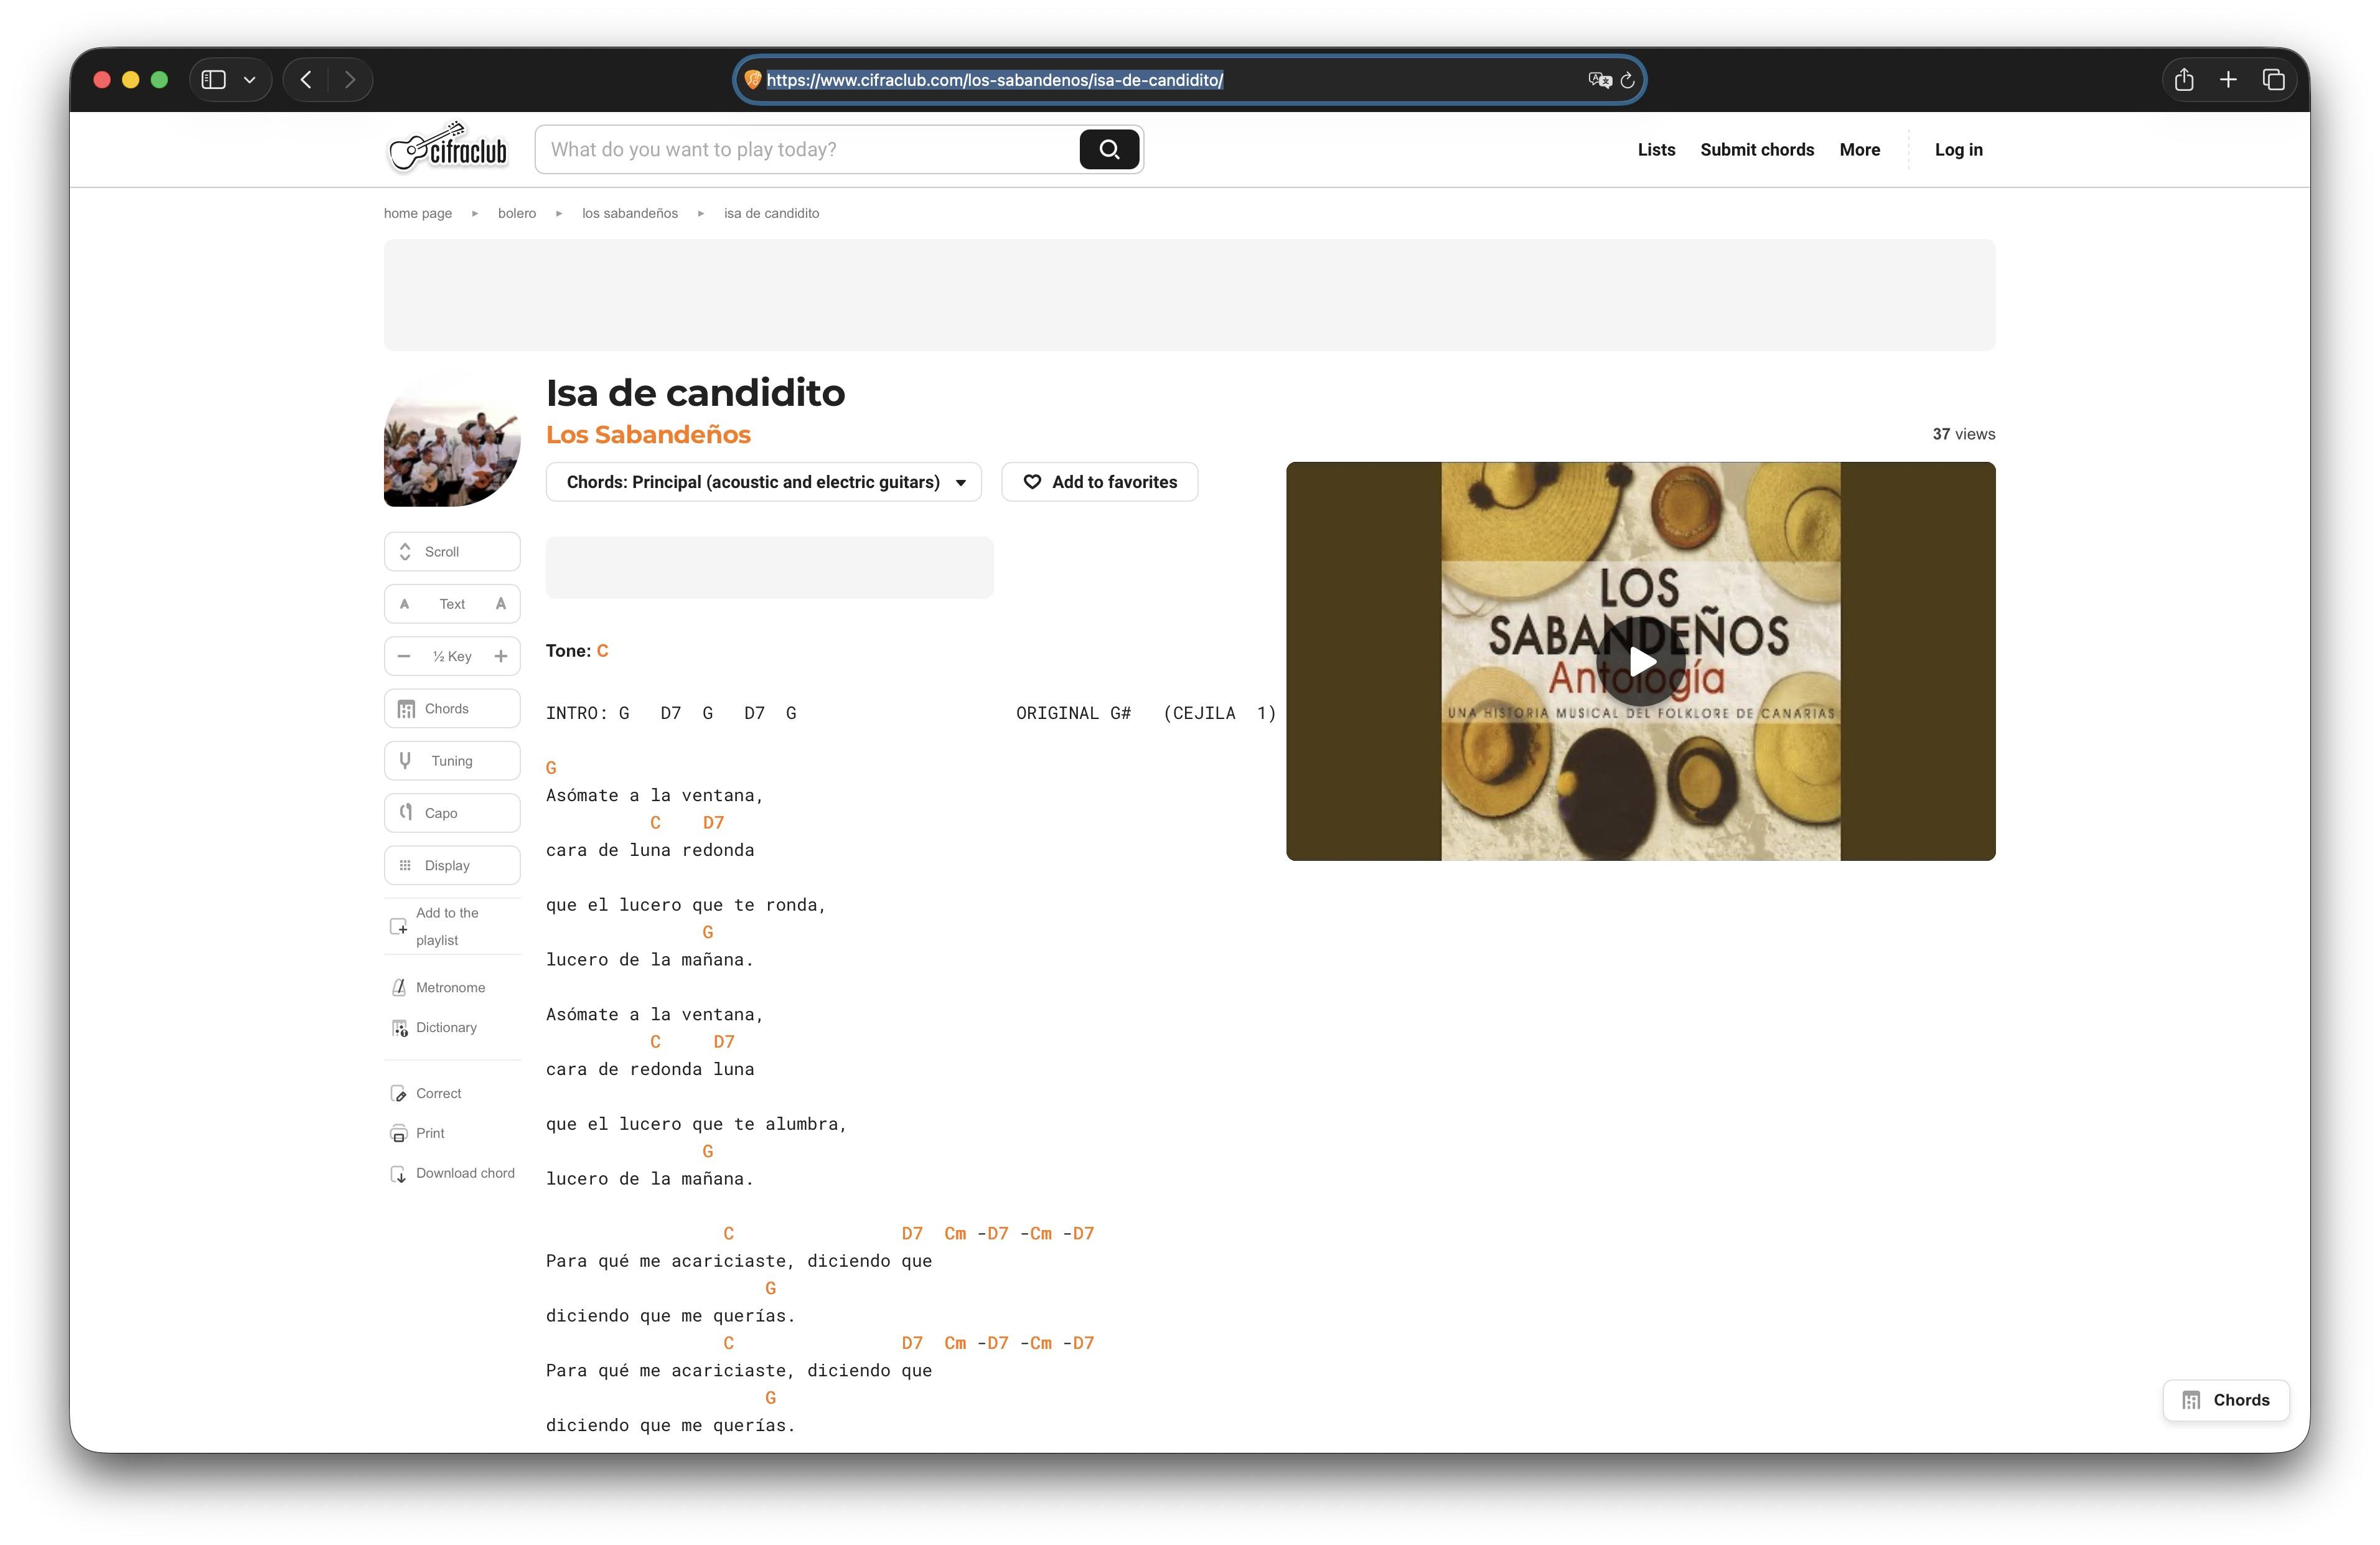
\includegraphics[width=0.80\textwidth]{Ilustraciones/estado/cifra_isadecandidito.jpeg}
    \caption{Letra y acordes de \emph{Isa de candidito} para guitarra en Cifra Club~\cite{cifra_isadecandidito}.}\label{fig:cifra_isadecandidito}
\end{figure}

Sin embargo, \textbf{el timple} no cuenta con las mismas facilidades. A diferencia de los instrumentos mencionados anteriormente, una simple búsqueda muestra cómo la información se encuentra dispersa en distintas plataformas, en su mayoría no especializadas:

\begin{itemize}
    \item \textbf{Redes Sociales}, siendo su principal medio de difusión. Podemos encontrar distintos perfiles, incluyendo comerciales \emph{(i.e. autores promocionando canciones, o profesores dando a conocer recursos o cursos de pago)}, así como perfiles didácticos y de aficionados. Destacamos a Raquel Álvarez que a través de la plataforma \textbf{YouTube} realiza una gran labor divulgativa mediante la enseñanza de técnicas para timple (véase Figura~\ref{fig:raquel_youtube_video}).
    
    \item \textbf{Páginas Web}, donde distinguimos:
    \begin{itemize}
        \item \textbf{Espacios dedicados a otros instrumentos}, con canciones que pueden ser reproducidas en el timple.
        \item \textbf{Páginas promocionales de cursos o recursos}, mayormente de pago. Destacamos a Pedro Izquierdo que a través de su página web ofrece servicios como cursos, herramientas y partituras (algunas gratuitas) (véase Figura~\ref{fig:pedro_izquierdo_pagina_partituras}).
    \end{itemize}
    
    \item \textbf{Libros}, mayormente físicos, de gran antigüedad o incluso inaccesibles actualmente.
\end{itemize}

\begin{figure}[H]
    \centering
    % Primera subfigura
    \begin{subfigure}[b]{0.48\textwidth}
        \centering
        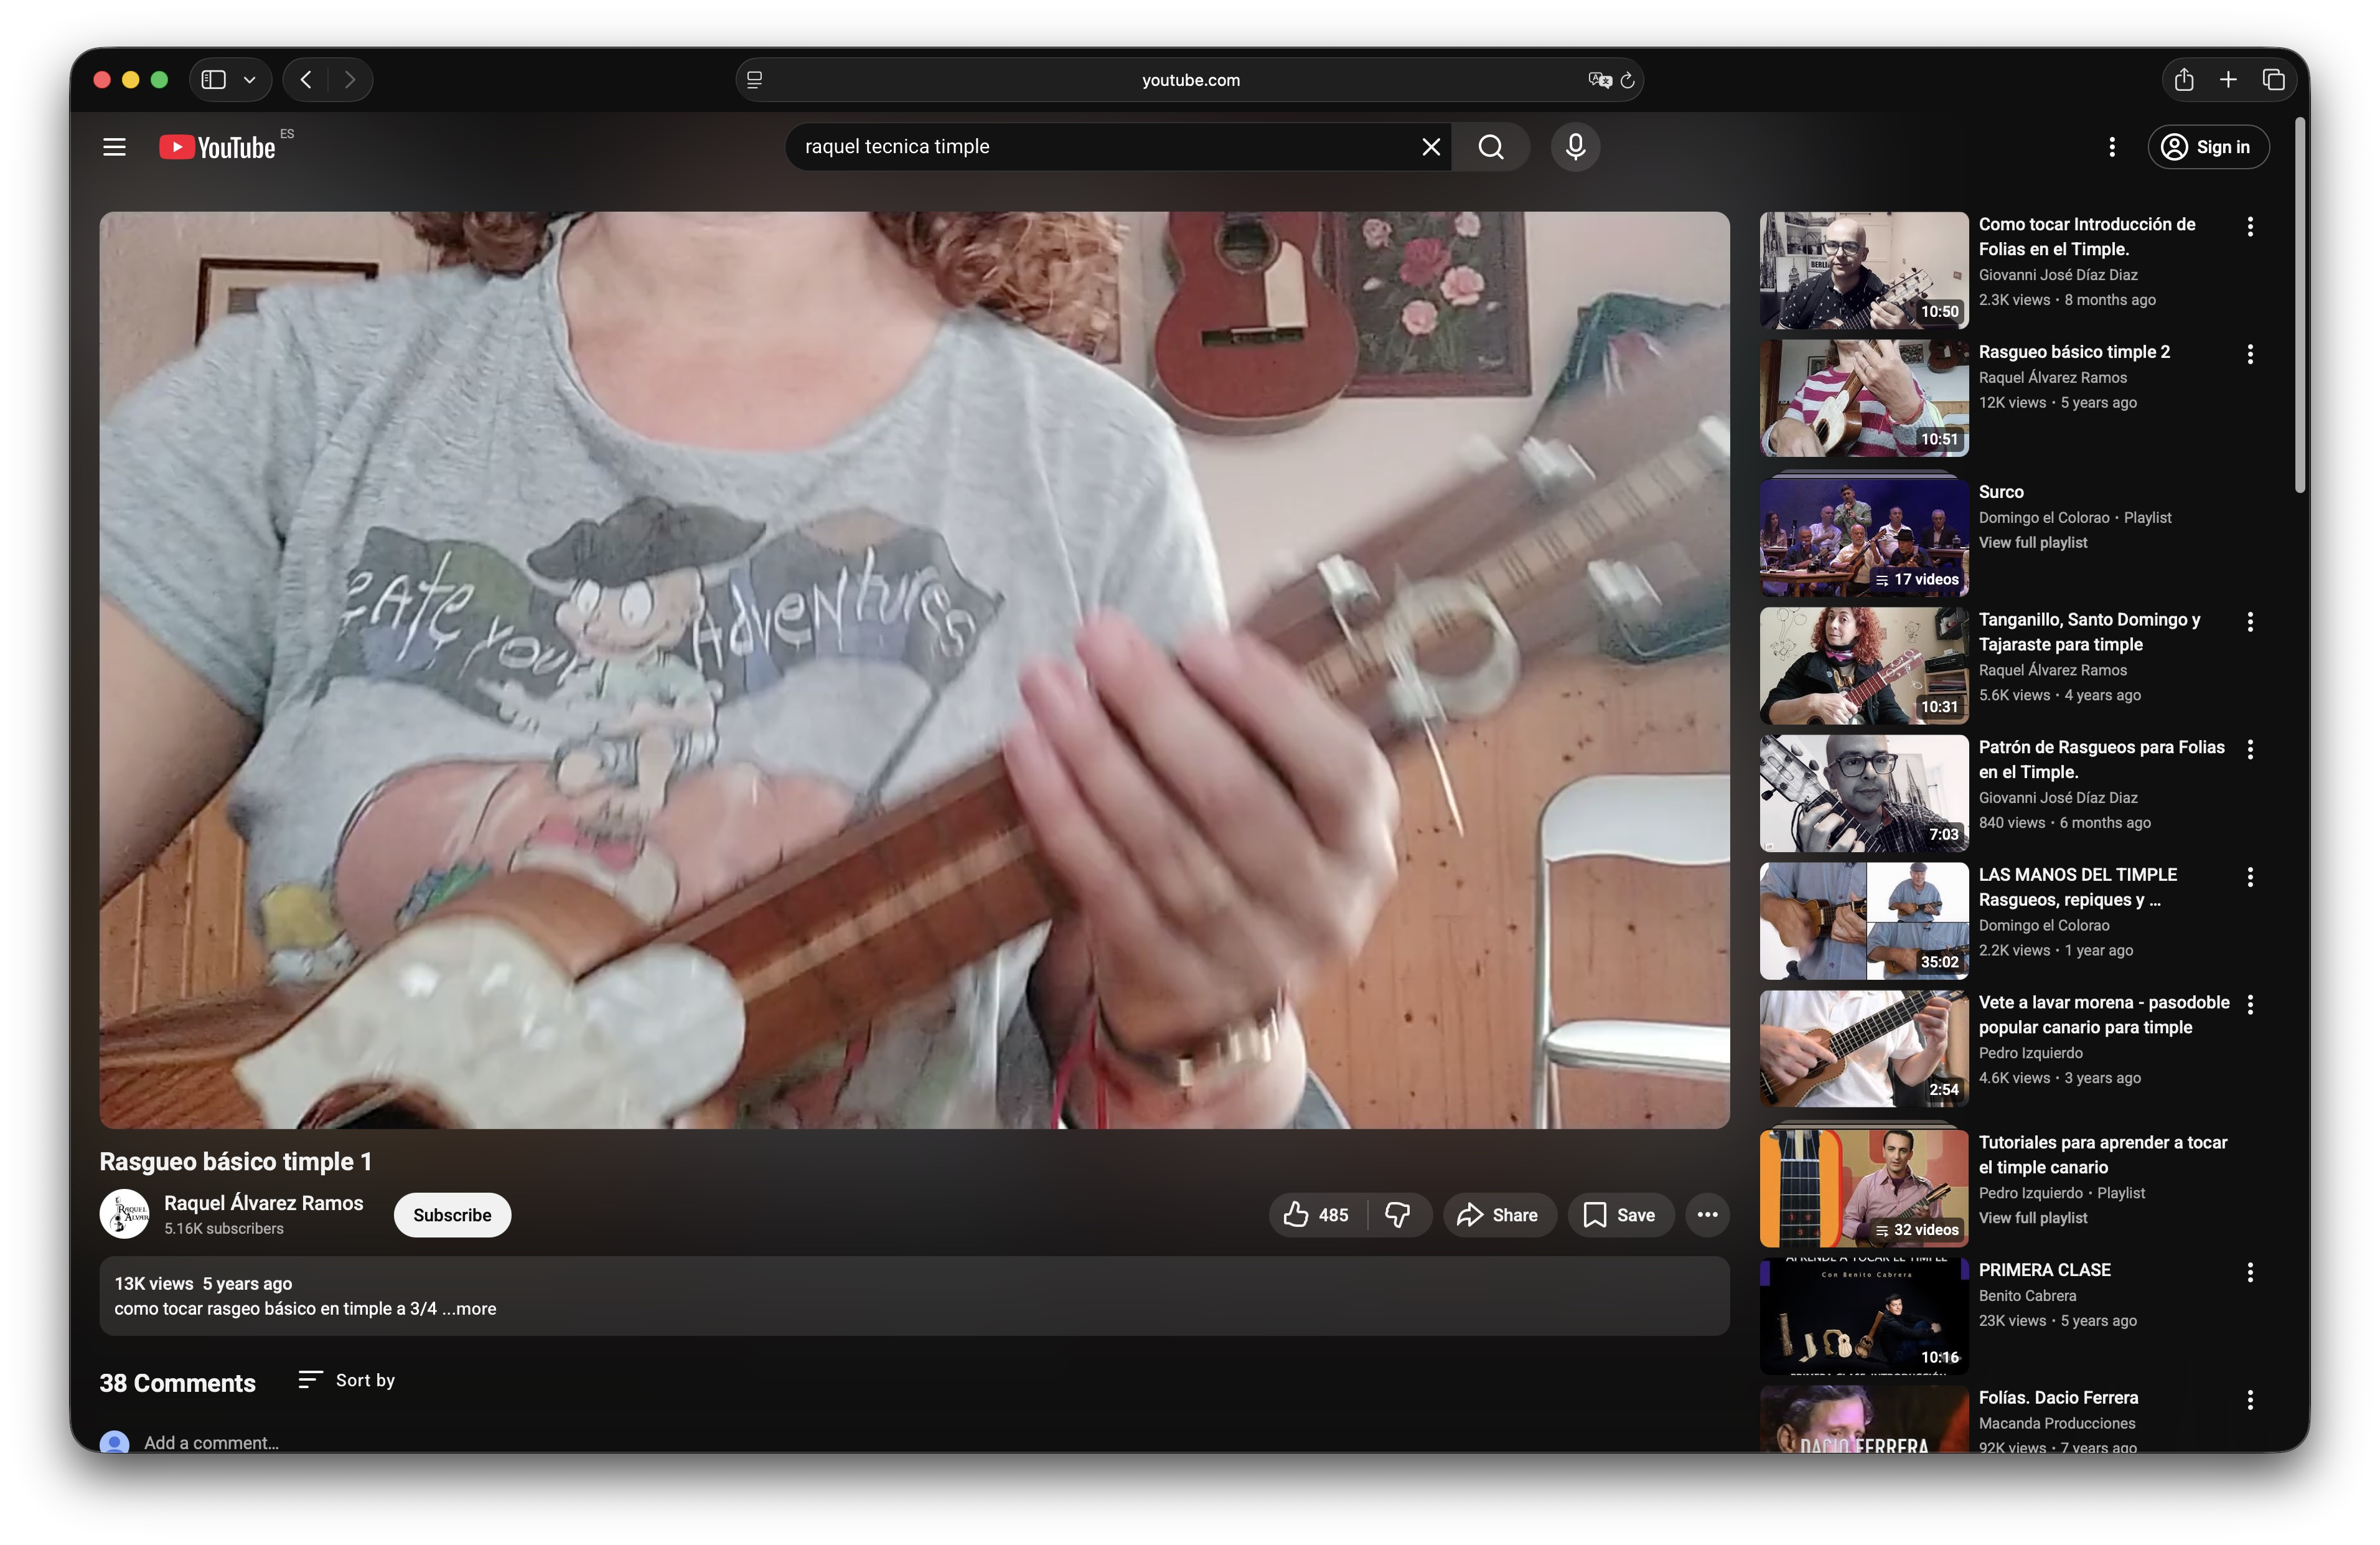
\includegraphics[width=\textwidth]{Ilustraciones/estado/raquel_youtube_video.jpeg}
        \caption{Video de \emph{Rasgueo básico timple 1} por Raquel Álvarez~\cite{raquel_youtube_video}}\label{fig:raquel_youtube_video}
    \end{subfigure}
    \hfill
    % Segunda subfigura
    \begin{subfigure}[b]{0.48\textwidth}
        \centering
        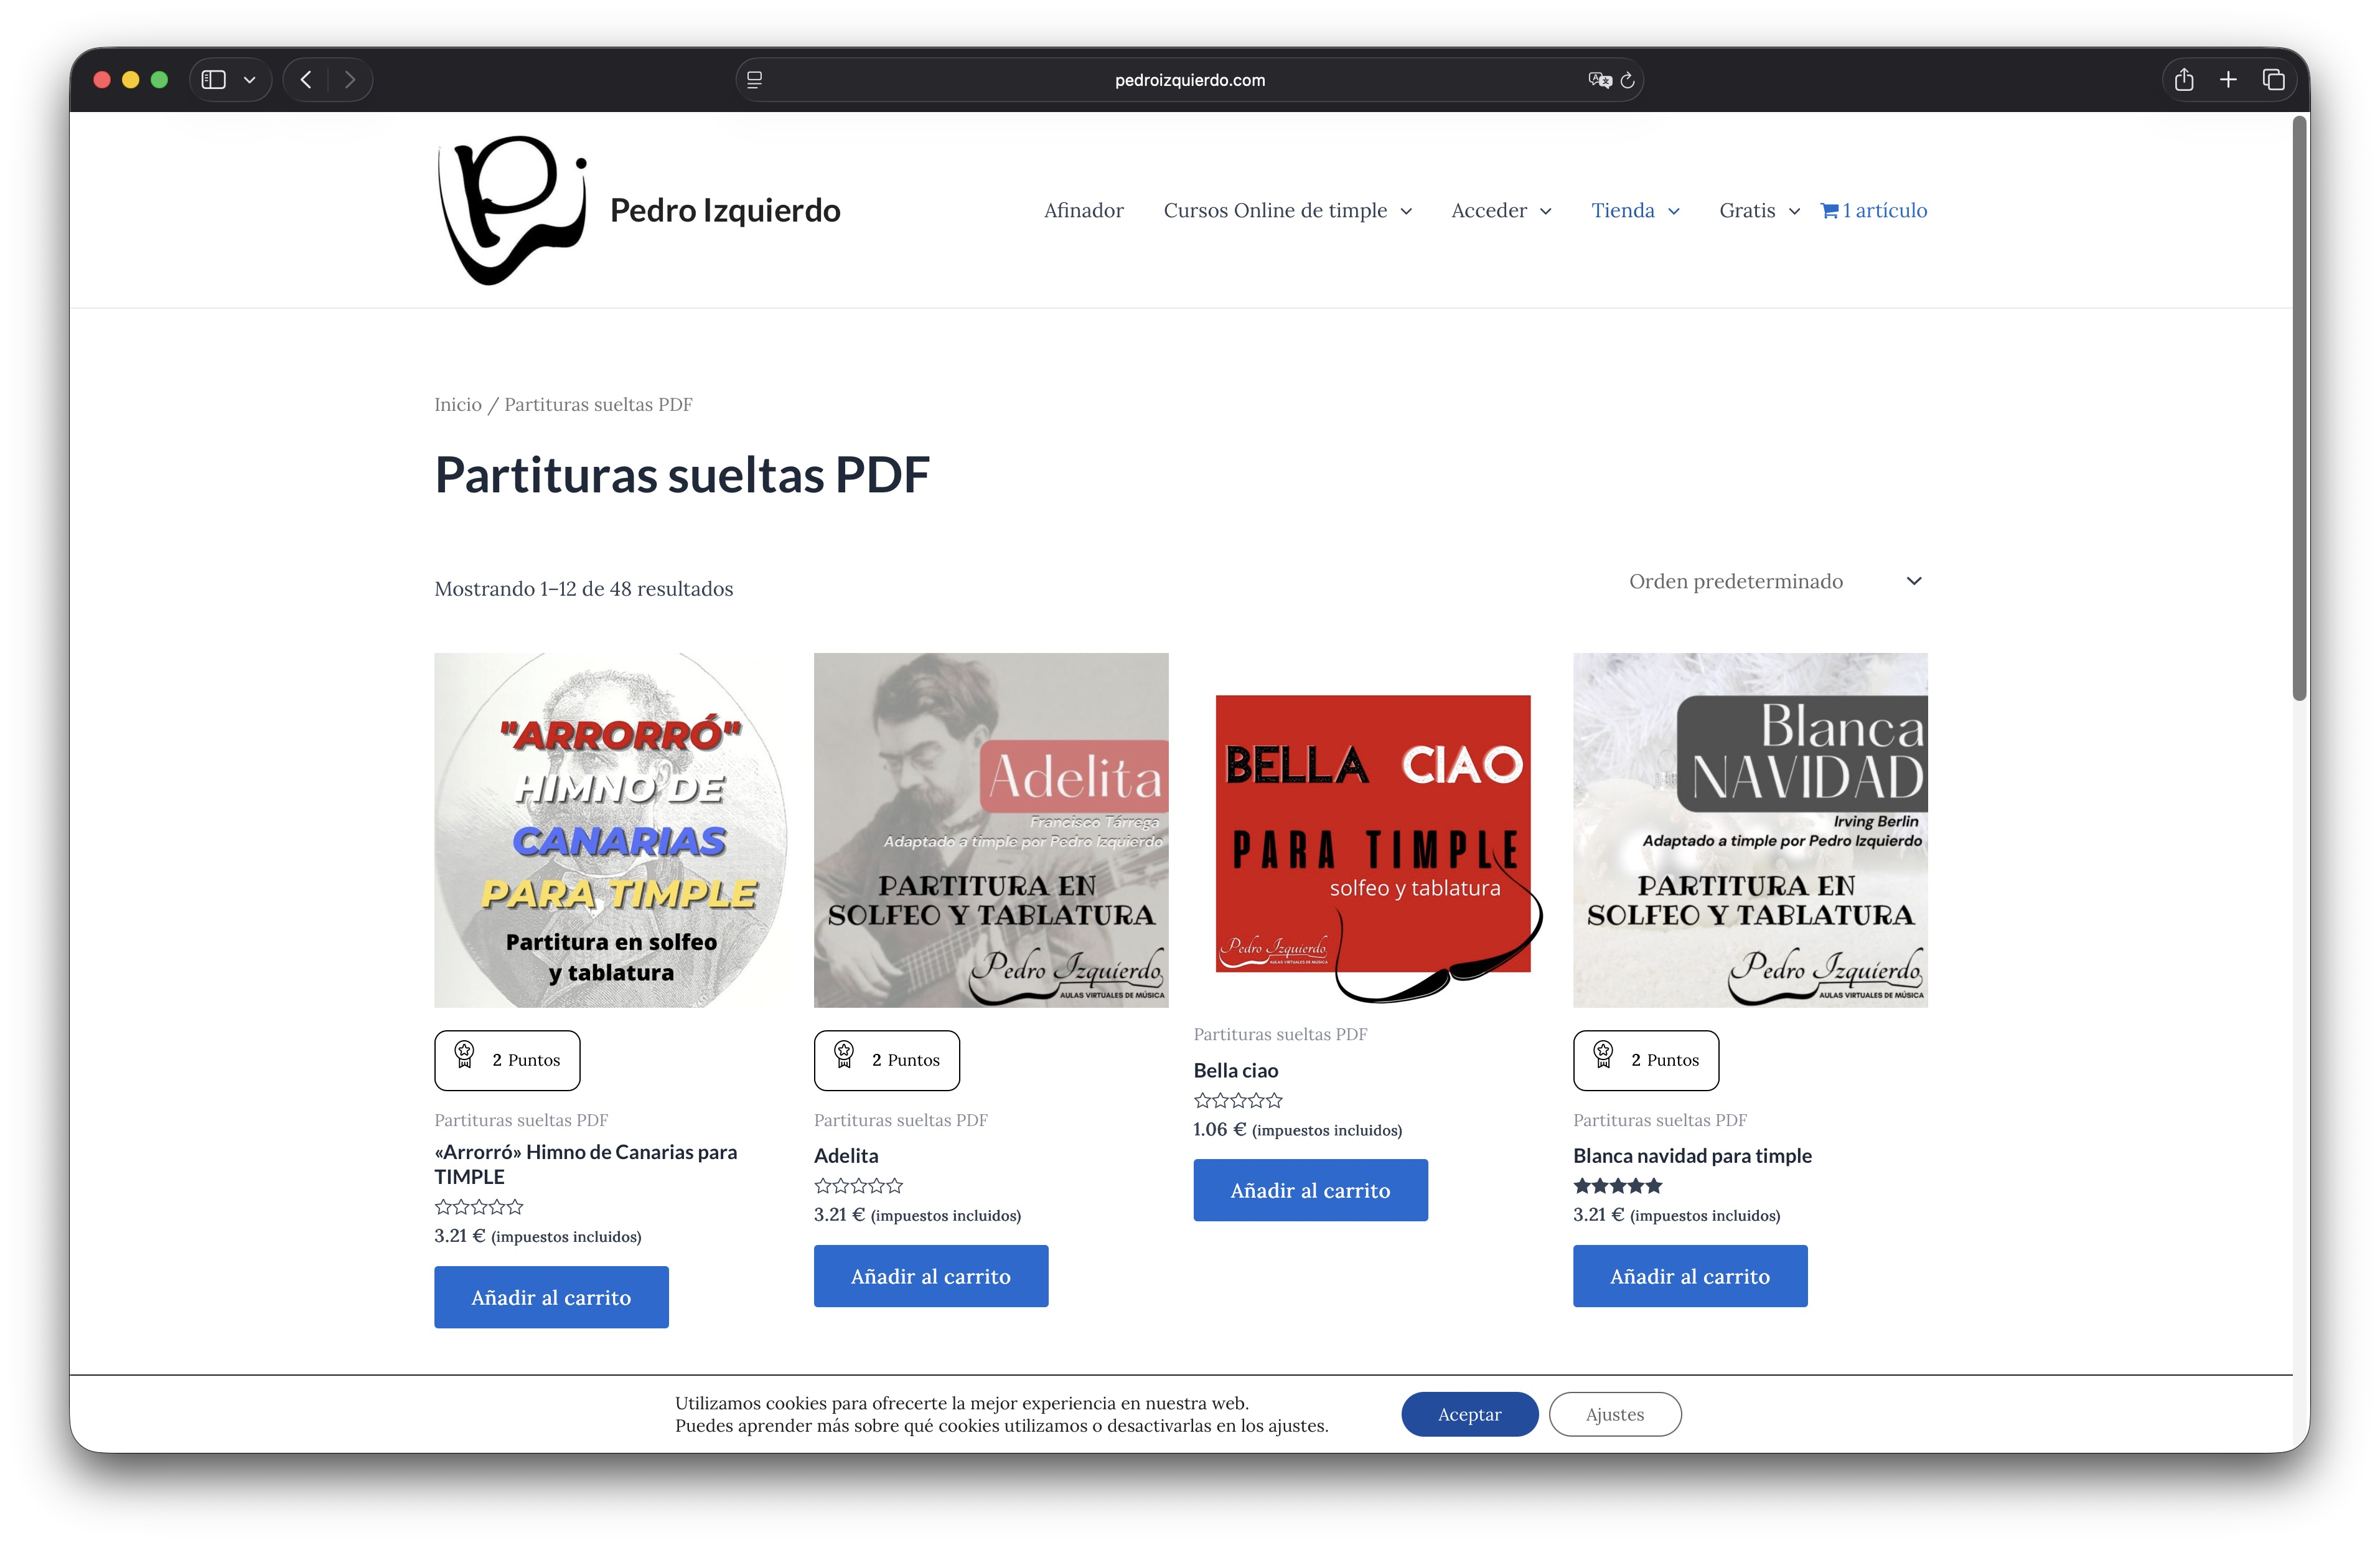
\includegraphics[width=\textwidth]{Ilustraciones/estado/pedro_izquierdo_pagina_partituras.jpeg}
        \caption{Partituras por Pedro Izquierdo en su página web~\cite{pedro_izquierdo_pagina_partituras}}\label{fig:pedro_izquierdo_pagina_partituras}
    \end{subfigure}
    % Caption general
    \caption{Recursos para timple en distintas plataformas digitales.}\label{fig:comparacion_timple}
\end{figure}

%Concluimos que, a diferencia de otros instrumentos, no existe un espacio digital dedicado exclusidamente al timple. Además, su comunidad se encuentra activa, pero dispersa en distintas plataformas. 

%Dada la escasez de alternativas y recursos, se abre la oportunidad de crear una aplicación web diseñada para el timple, poniendo a su comunidad como foco y ofreciendo todas las utilidades necesarias para la creación, difusión y práctica de canciones.

En conclusión, la comunidad del timple se encuentra fragmentada en distintas plataformas, con escasos recursos (en algunos casos antiguos o incluso inaccesibles) y sin un espacio propio. Estas necesidades no cubiertas y la existencia de alternativas exitosas para otros instrumentos, abren paso a la oportunidad para la creación de una aplicación web especificamente diseñada para este instrumento.